\subsection{Общие сведения о нейронных сетях}
% todo what is nn
\subsubsection{Многослойный перцептрон}
Описанный Фрэнком Розенблаттом перцептрон -- это линейная модель классификации.
Она делит пространство входов нейронной сети на две части гиперплоскостью\cite{Rosenblatt1958}.

Перцептрон состоит из элементов трех видов: сенсорные, ассоциативные и
реагирующие. Сенсорные элементы вырабатывают сигнал под воздействием энергии.
Ассоциативные элементы выдают сигнал, когда алгебраическая сумма входящих
сигналов превышает пороговую величину $\theta > 0$. Реагирующий элемент выдает
сигнал $+1$, если сумма входных его сигналов строго положительна, и $-1$, если
сумма входных сигналов строго отрицательная.
\begin{figure}[h]
\centering
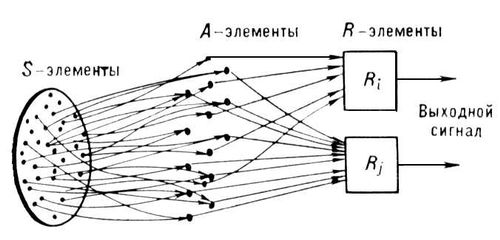
\includegraphics[width=0.5\textwidth]{Perceptron2}
\caption{Перцептрон. Источник: \url{http://www.machinelearning.ru/wiki/index.php?title=Изображение:Perceptron2.jpg}}
\label{fig:perceptron}
\end{figure}
\subsubsection{Свёрточные нейронные сети}
Свёрточные нейронные сети часто применяются в задачах распознавания образов.
Главной составляющей СНС является слой свертки.

Основная идея свёрточной сети -- обработка участка изображения независимо от
его положения. Слой свертки проходит <<окном>> по изображению и пытается
выделить признаки, строя их карту. Более строго этот процесс можно записать
с помощью формулы:
\[
y^{l}_{i, j} = \sum_{-d \leq a, b \leq d} W_{a,b}x^l_{i + a, j + b},
\]
где $y^l_{i, j}$ -- результат свертки на уровне $l$, а $x^l_{i, j}$ её вход (т.е.
выход предыдущего слоя), $W$ -- матрица весовых коэффициентов\cite{deeplearning}. 
На рисунке \ref{fig:conv_calc} продемонстрирован пример подсчета результата по 
данной формуле.
\begin{figure}[h]
\centering
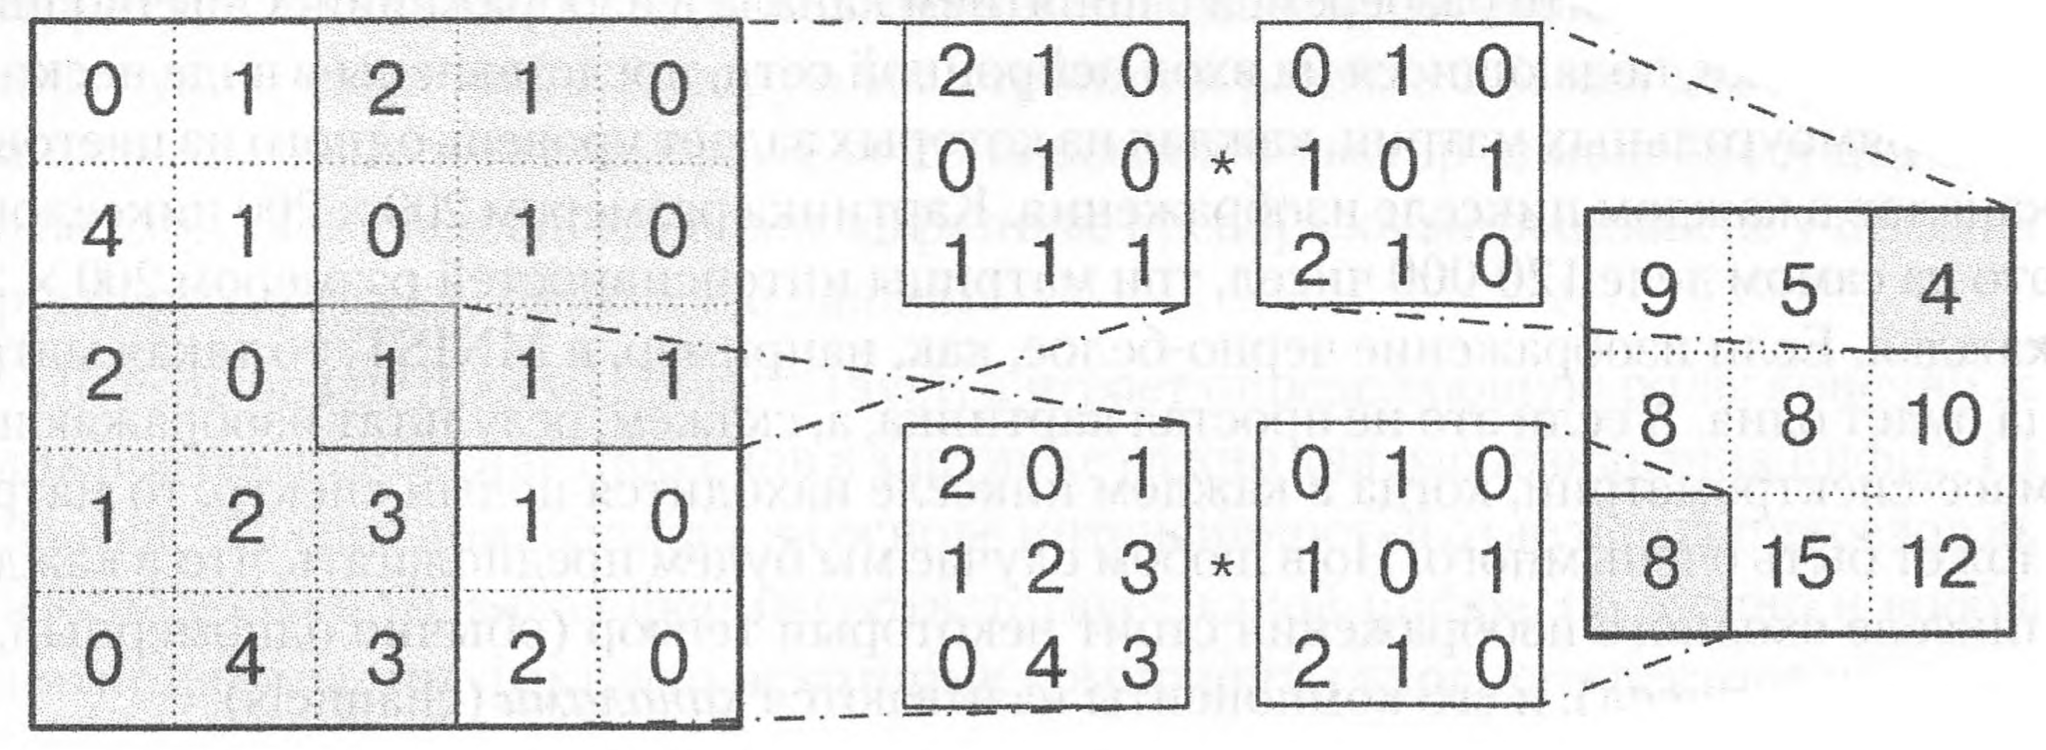
\includegraphics[width=0.8\textwidth]{conv_calc}
\caption{Пример подсчета результата свертки. Источник: \cite{deeplearning}}
\label{fig:conv_calc}
\end{figure}

Часто после операции свёртки добавляется ещё одна операция, называемая
субдискретизацией (англ. \textit{pooling}). Существуют различные вариации данной
операции, но чаще всего применяется операция взятия максимума:
\[
x^{l+1}_{i,j} = \max_{{-d \leq a \leq d, -d \leq b \leq d}} z^{l}_{i+a, j+b}.
\]
Связано это с тем, что как правило важно само наличие признака, а не его точные
координаты\cite{deeplearning}.

Пионером свёрточных сетей считается научная группа Яна Лекуна, представившая в
1998 году архитектуру LeNet-5. Подробно она описывается в работе \cite{LeCun}.

\begin{figure}[h]
\centering
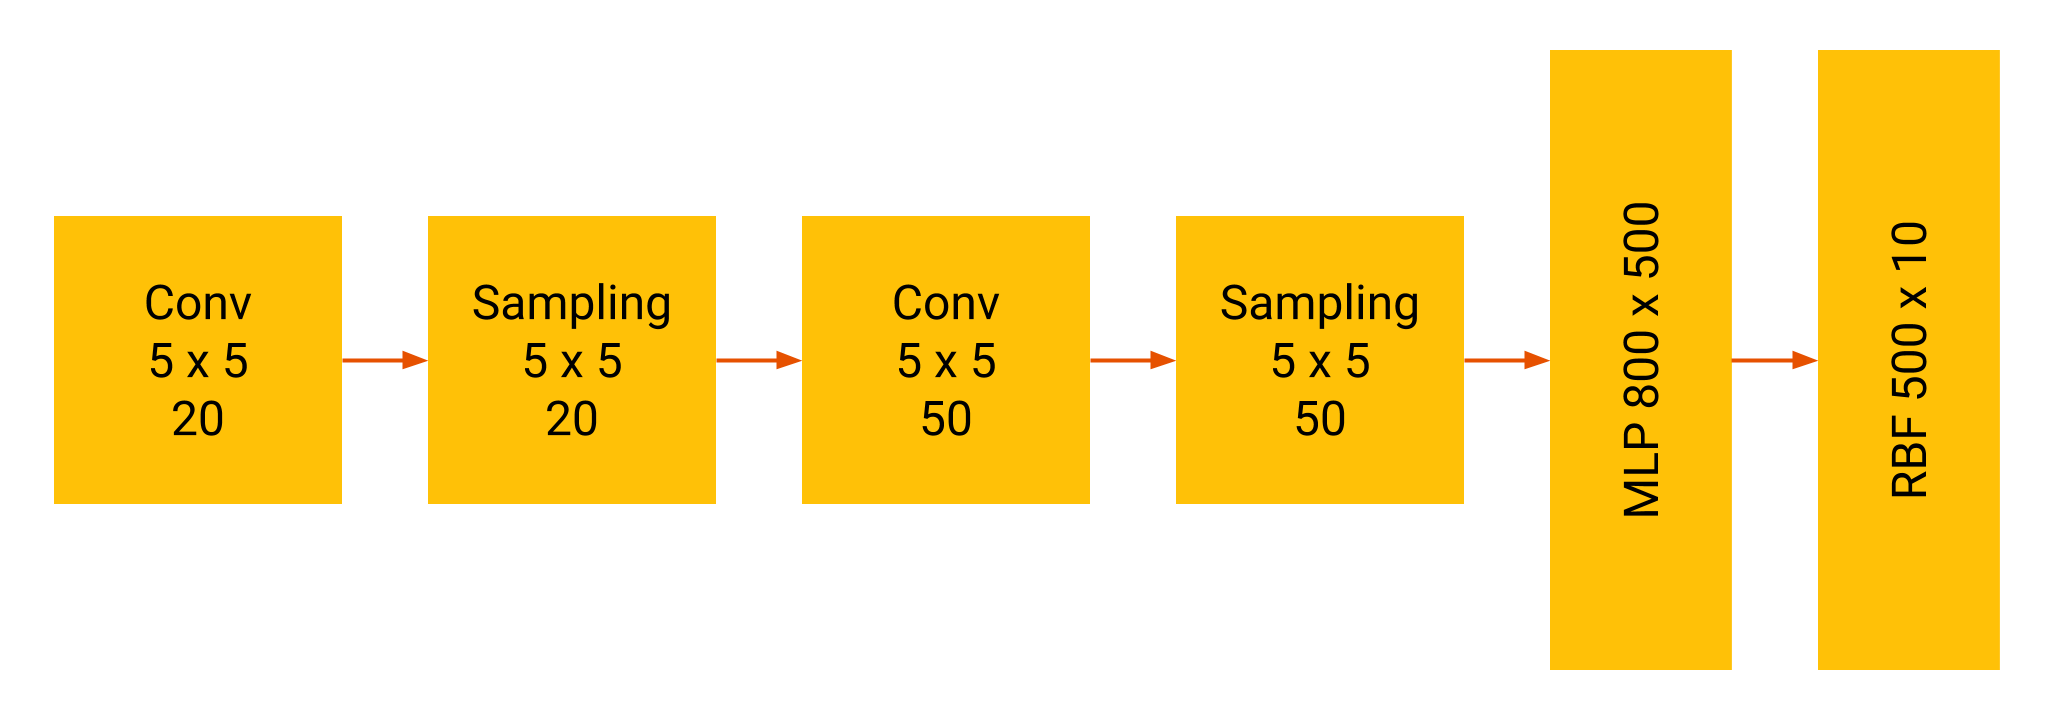
\includegraphics[width=0.8\textwidth]{LeNet}
\caption{LeNet-5}
\label{fig:lenet}
\end{figure}

\subsubsection{Рекуррентные нейронные сети}
Часто исходными данными для нейронных сетей служат последовательности, имеющие
зависимости соседних точек друг от друга. Для выражения такой зависимости
применяются рекуррентные нейронные сети, где связи могут идти не только от
нижнего слоя к верхнему, но и от нейрона к самому себе. 

\begin{figure}[h]
\centering
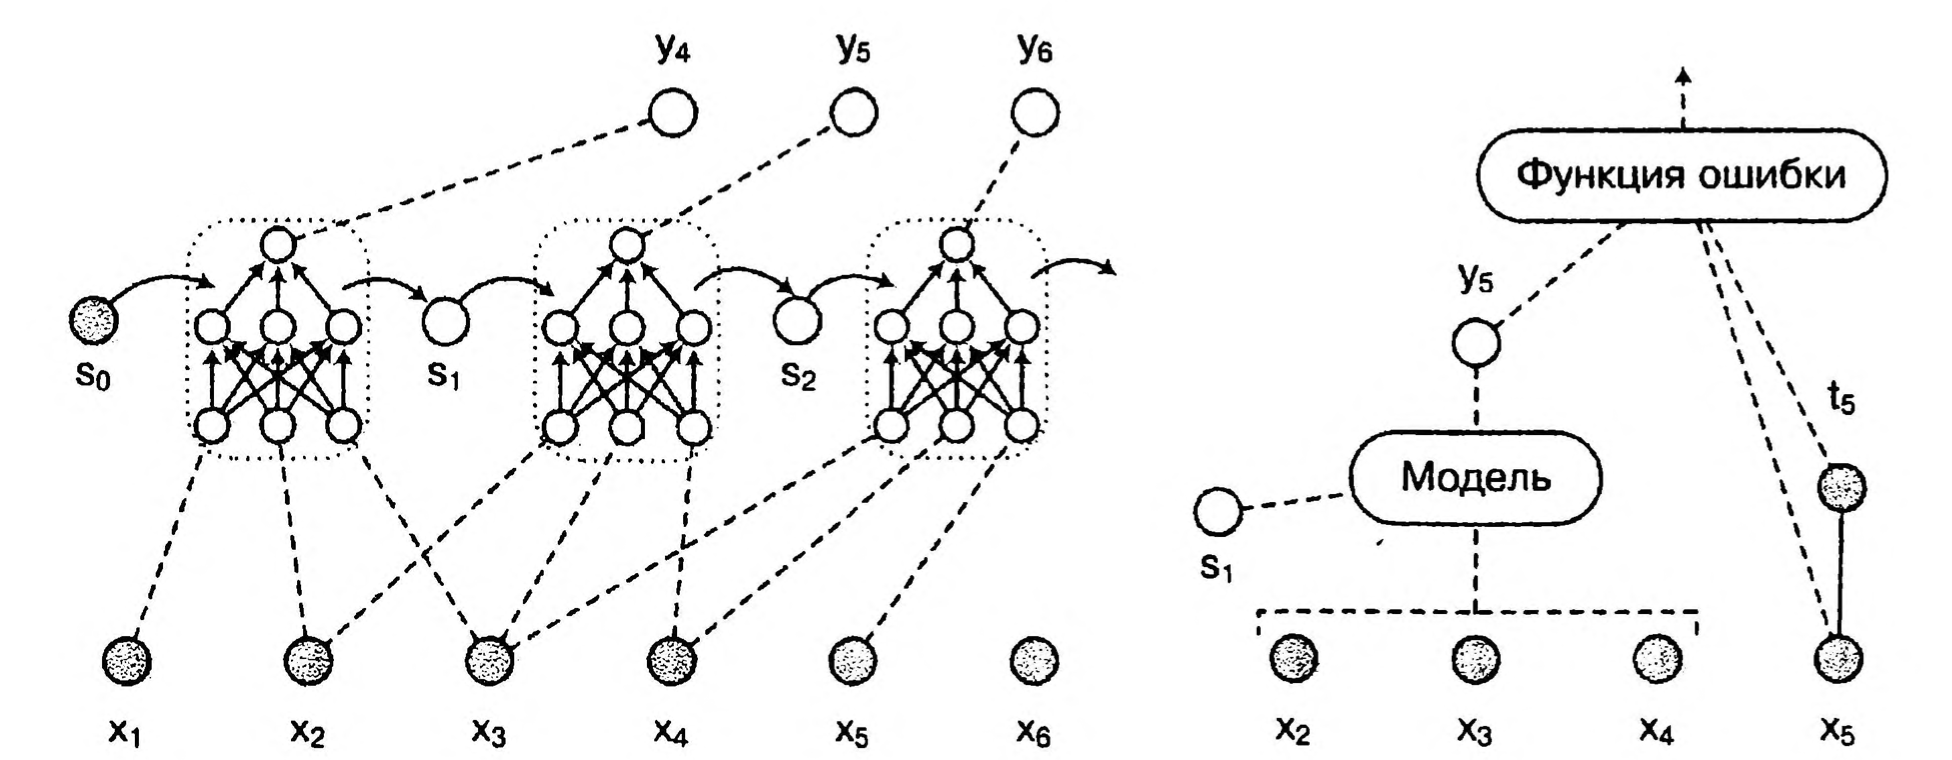
\includegraphics[width=0.8\textwidth]{recurrent_network}
\caption{Рекуррентная нейронная сеть. Источник: \cite{deeplearning}}
\label{fig:recurrent_network}
\end{figure}

На практике часто используется архитектура Long Short-Term Memory (LSTM). Она
состоит из трёх основных видов узлов (вентилей): входной, забывающий и выходной.
На вход ей подаются два вектора: вектор входных данных $x_t$ и вектор скрытого
состояния $h_{t-1}$. Внутри каждого блока есть векторы, выполняющий функцию
памяти (ячейка памяти)\cite{deeplearning}. Это демонстрирует схема на рис.~\ref{fig:lstm}.
Впервые архитектура LSTM была описана в работе \cite{Hochreiter1997}.
\begin{figure}[h]
\centering
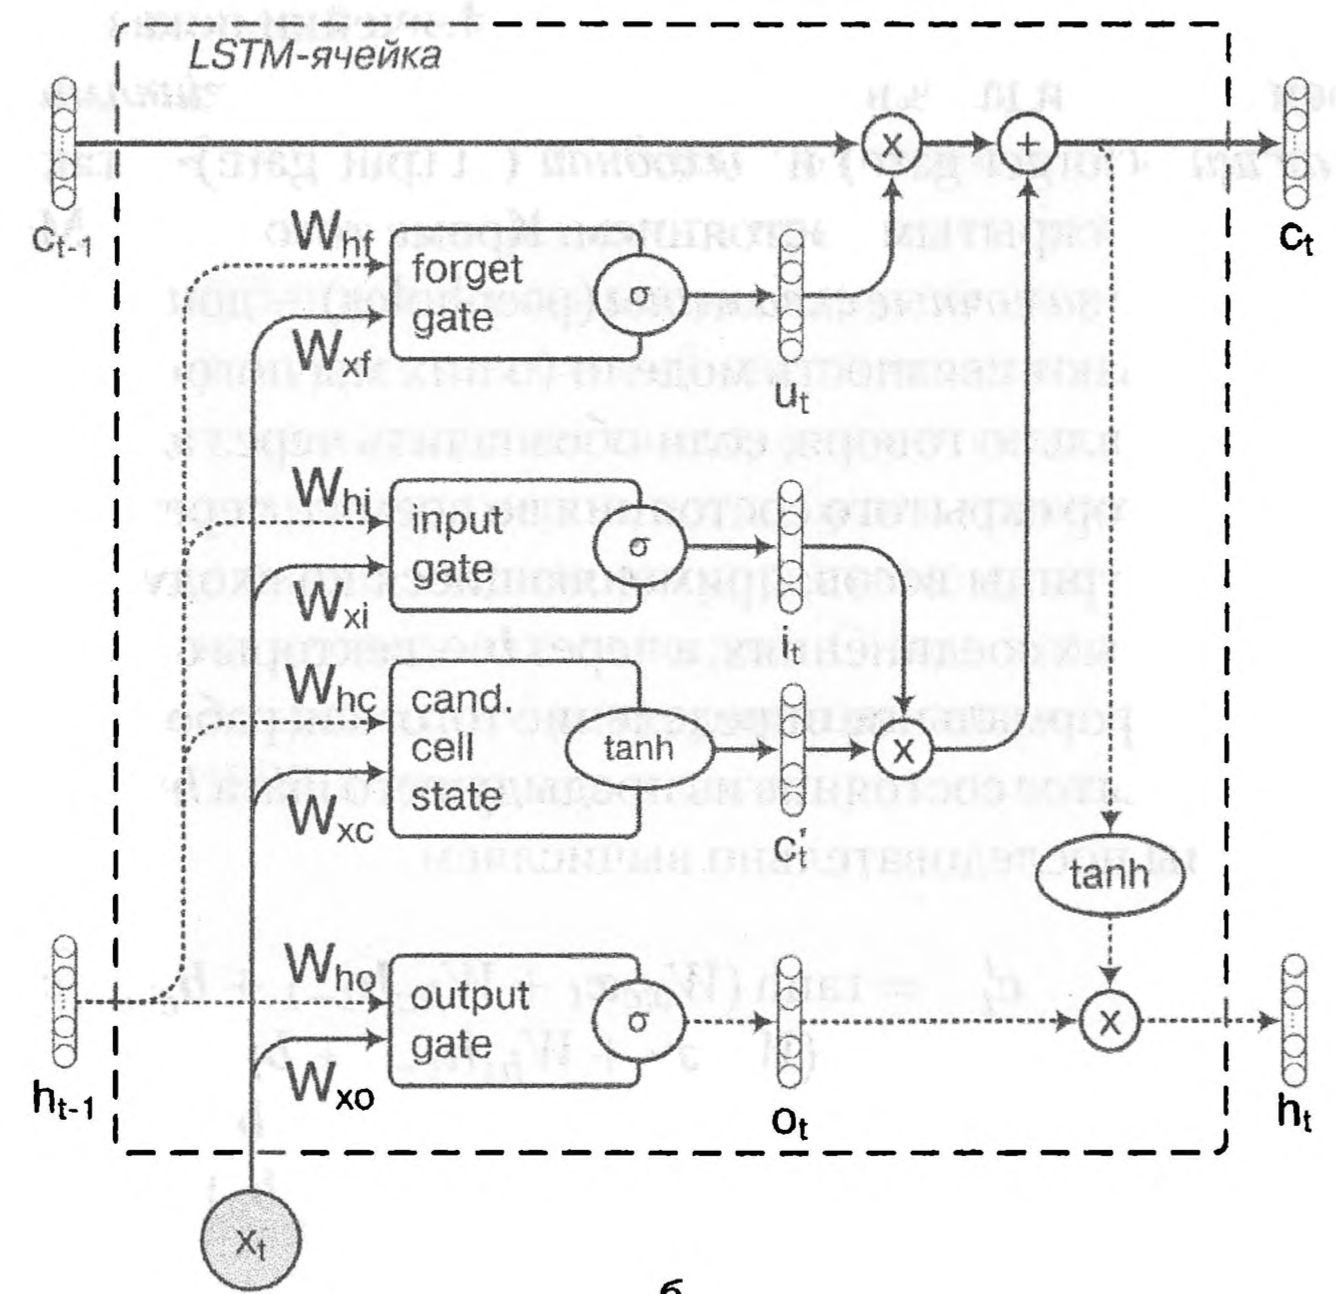
\includegraphics[width=0.8\textwidth]{lstm}
\caption{Ячейка LSTM. Источник: \cite{deeplearning}}
\label{fig:lstm}
\end{figure}

\subsubsection{Граф вычислений}
Об обучении нейронной сети можно думать как о задаче глобальной оптимизации
некоторой функции. В свою очередь, удобным способом представления функции
является граф вычислений.

Граф вычислений -- это граф, узлами которого являются функции, а ребра связывают
функции со своими аргументами\cite{deeplearning}. Это можно продемонстрировать
на следующем примере:
\begin{equation}
f(x, y) = x^2 + xy + (x + y)^2
\label{eq:graph_sample_f}
\end{equation}

Для данной функции можно построить три эквивалентных графа вычислений (см.
рис. \ref{fig:graph_for_f}). Если функции в вершинах достаточно просты, чтобы
взять от них производную, то не составит труда взять производную всей функции,
представленной этим графом, воспользовавшись правилами дифференцирования сложной
функции. Это, в свою очередь, позволяет применить для обучения метод градиентного
спуска, а точнее, одну из его модификаций -- метод обратного распространения
ошибки. Основная его идея состоит в распространении сигналов ошибки
от выходов сети к входам в направлении, обратном прямому распространению
сигнала.

\begin{figure}[h]
\centering
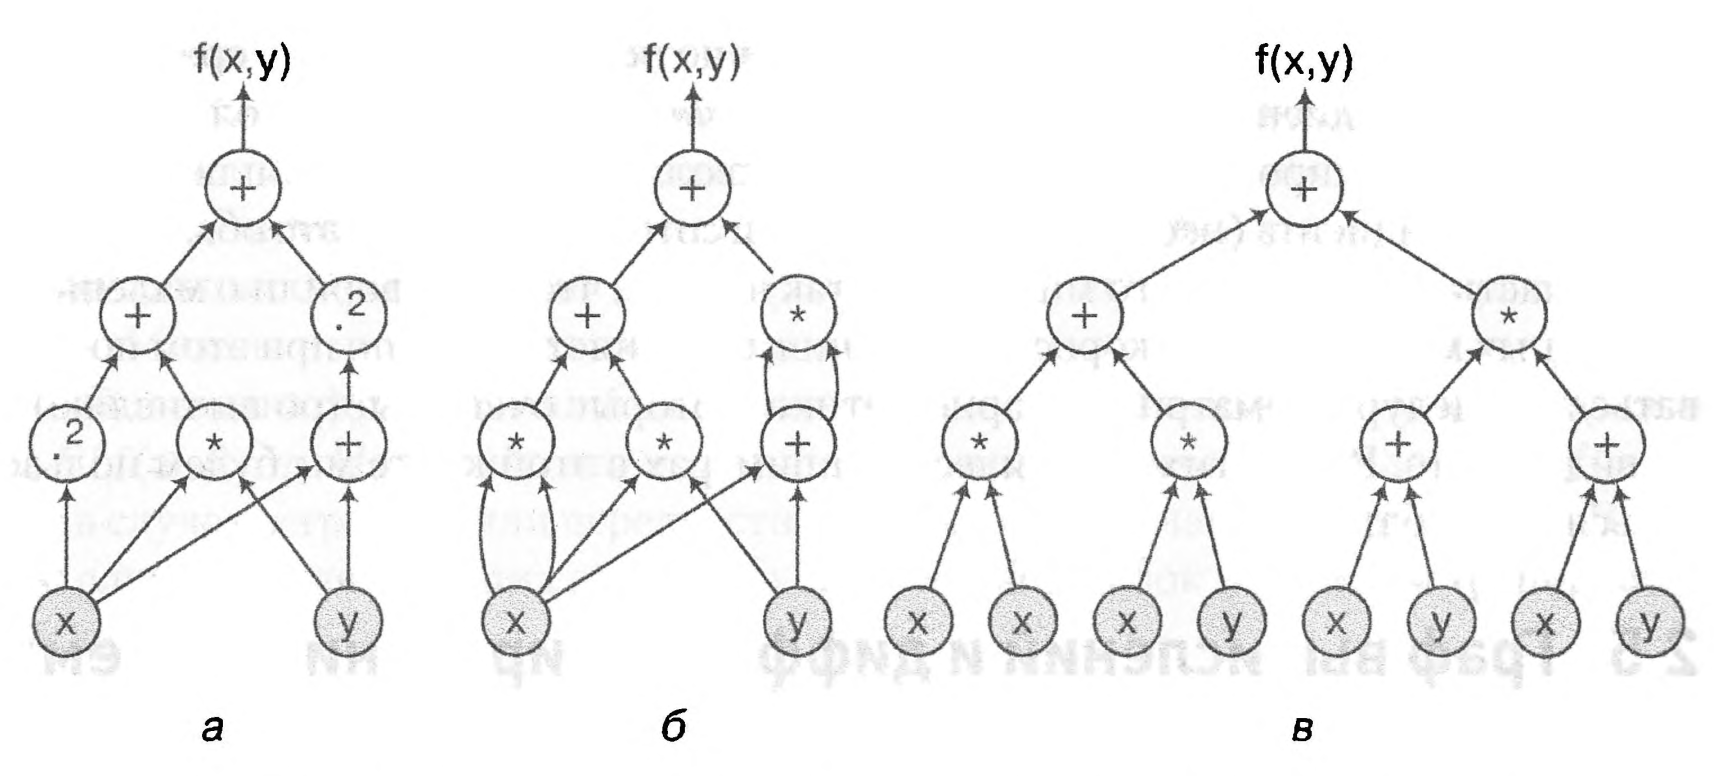
\includegraphics[width=0.8\textwidth]{graph_f}
\caption{Три графа вычислений для (\ref{eq:graph_sample_f}). Источник: \cite{deeplearning}}
\label{fig:graph_for_f}
\end{figure}
